\section{Zielsetzung}
Bei dem im folgenden durchgeführten Versuch wurde die Beugung von Licht untersucht. Zu diesem Zweck wurde sowohl für einen Einzel als 
auch für einen Doppelspalt das Interferenzmuster durch Intensitätsmessungen aufgenommen.
\section{Theorie}
Wenn Licht auf einen Spalt oder ein undurchlässiges Objekt mit einer Länge kleiner dem Strahldurchmesser trifft kommt es zu Beugungserscheinungen,
das Licht ändert also seine Ausbreitungsrichtung in einer Art, die von der üblichen Beschreibung der geometrischen Optik durch Lichtstrahlen
abweicht. Dieses Phänomen lässt sich im Zuge des Welle-Teilchen-Dualismus am besten mithilfe des Wellenmodells des Lichts erklärt werden.
Wenn Licht in Näherung durch das klassische Wellenmodell beschrieben wird, kann die Beugung durch das sogenannte Huygenssche Prinzip erklärt werden,
welches besagt, dass jeder Punkt der Welle am Spalt, bzw. allgemein am beugenden Objekt, als Augangspunkt einer Elementarwelle betrachtet werden kann, welche 
sich Kugelförmig im Raum ausbreitet. \\
Bei der Beobachtung von Lichtbeugung am Spalt wird grundsätzlich zwischen zwei Versuchsanordnungen unterschieden: 
\begin{figure} [h]
    \centering
    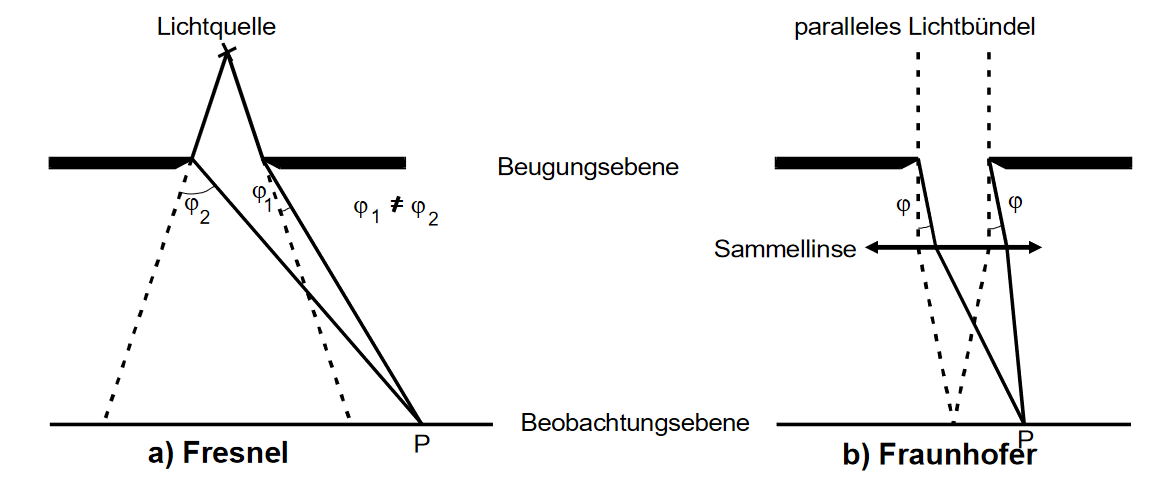
\includegraphics[width=14cm, keepaspectratio]{Beugungsanordnungen}
    \caption{Beugungsanordnungen}
 \end{figure}
Zum einen der Fresnelschen Anordnung, bei der
Lichtquelle und Schirm im endlichen liegen, sodass die Strahlen divergent sind. Bei dieser Anordnung interferien am Punkt $P$ Strahlen unter
unterschiedlichen Beugungswinkeln. \\ Im Gegensatz dazu wird bei der Fraunhoferschen Anordnung sowohl die Lichtquelle als auch der Aufpunkt
ins Unendliche verlegt, wobei letzteres in der Praxis meist durch eine Sammellinse erreicht wird. Dies führt dazu, dass parallele Strahlenbündel
auf den Spalt treffen. Da in diesem Fall Strahlen interferieren, die unter identischen Winkeln abgebeugt werden, ist diese Form der Beugung wesentlich 
einfacher zu behandeln als die Fresnelsche und wird daher auch in diesem Experiment verwendet. \\
Wenn eine Welle der Feldstärke
\begin{equation}
A(z,t)=A_0\exp(i(wt-2\pi z/\lambda))
\end{equation}
auf einen Spalt der Breite $b$ fällt, sendet gemäß dem Huygensschen Prinzip wie oben geschildert jeder Punkt der Wellenfront
eine Elementarwelle aus.
\begin{figure} [h]
    \centering
    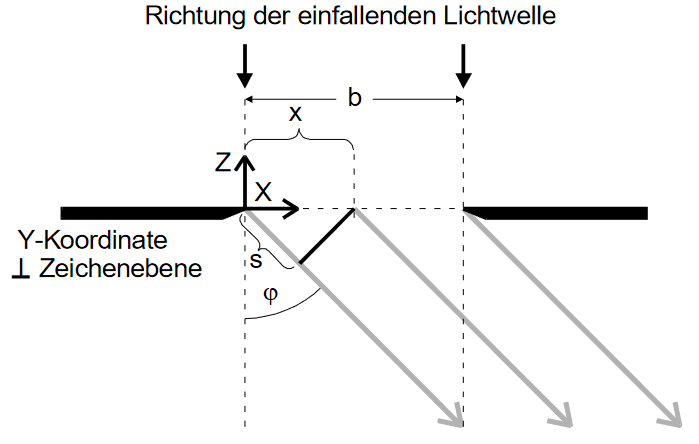
\includegraphics[height=7cm, keepaspectratio]{Spalt geometrie}
    \caption{Geometrie am Spalt}
 \end{figure}
Diese können aufgrund ihrer Kohärenz miteinander interferieren und bilden eine Welle, welche der Einhüllenden der Elementarwellen 
entspricht. \\ Zur Bestimmung des Beugungsbildes muss nun über alle unter dem gleichen Winkel $\phi$ abgebeugten Strahlen 
integriert werden. Aus geometrischen Beziehungen lässt sich herleiten, dass für die Weglängendifferenz zum Aufpunkt $P$ zweier solcher Strahlenbündel mit Abstand $x$ gilt:
\begin{equation}
s=xsin(\phi)
\end{equation}
Daraus lässt sich auch die Phasendifferenz der Wellenfronten bestimmen. Diese ergibt sich zu
\begin{equation}
\delta=2\pi\frac{s}{\lambda}=\frac{2\pi xsin(\phi)}{\lambda}
\end{equation}
Mit einem Integral über die gesamte Spaltbreite der Form
\begin{equation}
B(z,t,\phi)=A_0 \int_{0}^{b} \exp(i(wt-\frac{2\pi z}{\lambda}+\delta))dx
\end{equation}
kann nun die Feldstärke $B$ in Abhängigkeit vom gebeugten Winkel bestimmt werden. Dies ergibt nach einigen weiteren Rechnungen eine 
Amplitudenverteilung der Form:
\begin{equation}
B(z,t,\phi)=A_0\exp(i(wt-\frac{2\pi z}{\lambda}))\exp(\frac{\pi ib\sin(\phi)}{\lambda})\frac{\lambda}{\pi \sin(\phi)}\sin(\frac{\pi b\sin(\phi)}{\lambda})
\end{equation}
wovon de Facto jedoch nur der letzte Term relevant für die Intensitätsmessung ist, da es sich bei den anderen
Termen lediglich um komplexe Phasenfunktionen handelt. Mithilfe der Einführung der Konstante $\eta=\pi b\sin(\phi)/\lambda$
lässt sich daher der relevante Term auf 
\begin{equation}
B(\phi)=A_0b\frac{\sin(\eta)}{\eta}
\end{equation}
mit Nullstellen an den Punkten
\begin{equation}
\sin(\phi_n)=\pm n\frac{\lambda}{b}
\end{equation}
verkürzen. Für die Messung muss auf die zeitlich gemittelte Intensität
\begin{equation}
    \label{eq:einfachspalt}
I(\phi)\propto B(\phi)^2=A_0^2b^2\frac{\sin^2(\eta)}{\eta^2}
\end{equation}
zurückgegriffen werden, da diese sich wesentlich einfacher messen lässt als die Amplitude. \\
Mit einer analogen Rechnung lässt sich auch der Doppelspalt beschreiben, welcher als eine Überlagerung zweier einzelner Spalte im Abstand $s$ verstanden
werden kann. Dies führt zu einer Intensitätsverteilung der Form
\begin{equation}
    \label{eq:doppelspalt}
I(\phi)\propto B(\phi)^2=4\cos^2(\frac{\pi s\sin(\phi)}{ \lambda })\frac{\sin^2(\eta)}{\eta^2}
\end{equation}
welche aus der ursprünglichen Verteilung des Eizelspaltes ergänzt um einen $\cos^2$ Term besteht.


